\chapter{Preliminaries}
\label{ch:preliminaries}

Starting from the basics, this chapter introduces the definitions and notation used in this work.

\section{Graph Classes}

A graph $G = (V, E)$ is defined by its vertices $V = \{ v_0, \ldots , v_n \}$ and edges $E \subseteq V \times V$. Though all our graphs are undirected, we use the edge notation $(v, w)$ for readability without implying a direction.

A \emph{drawing} of a graph is a representation of the vertices and edges of $G$ in the plane. A drawing contains an implied mapping of every graph vertex to a planar x-/y-coordinate, and of every edge to a curve such that the endpoints of the curve are the planar coordinates of the incident vertices.

A graph $G$ is \emph{planar} if there exists a drawing of $G$ such that none of the curves, which represent the edges, intersect or overlap. All \emph{trees}---cycle-free connected graphs---are planar.

\begin{figure}[t]
    \centering
    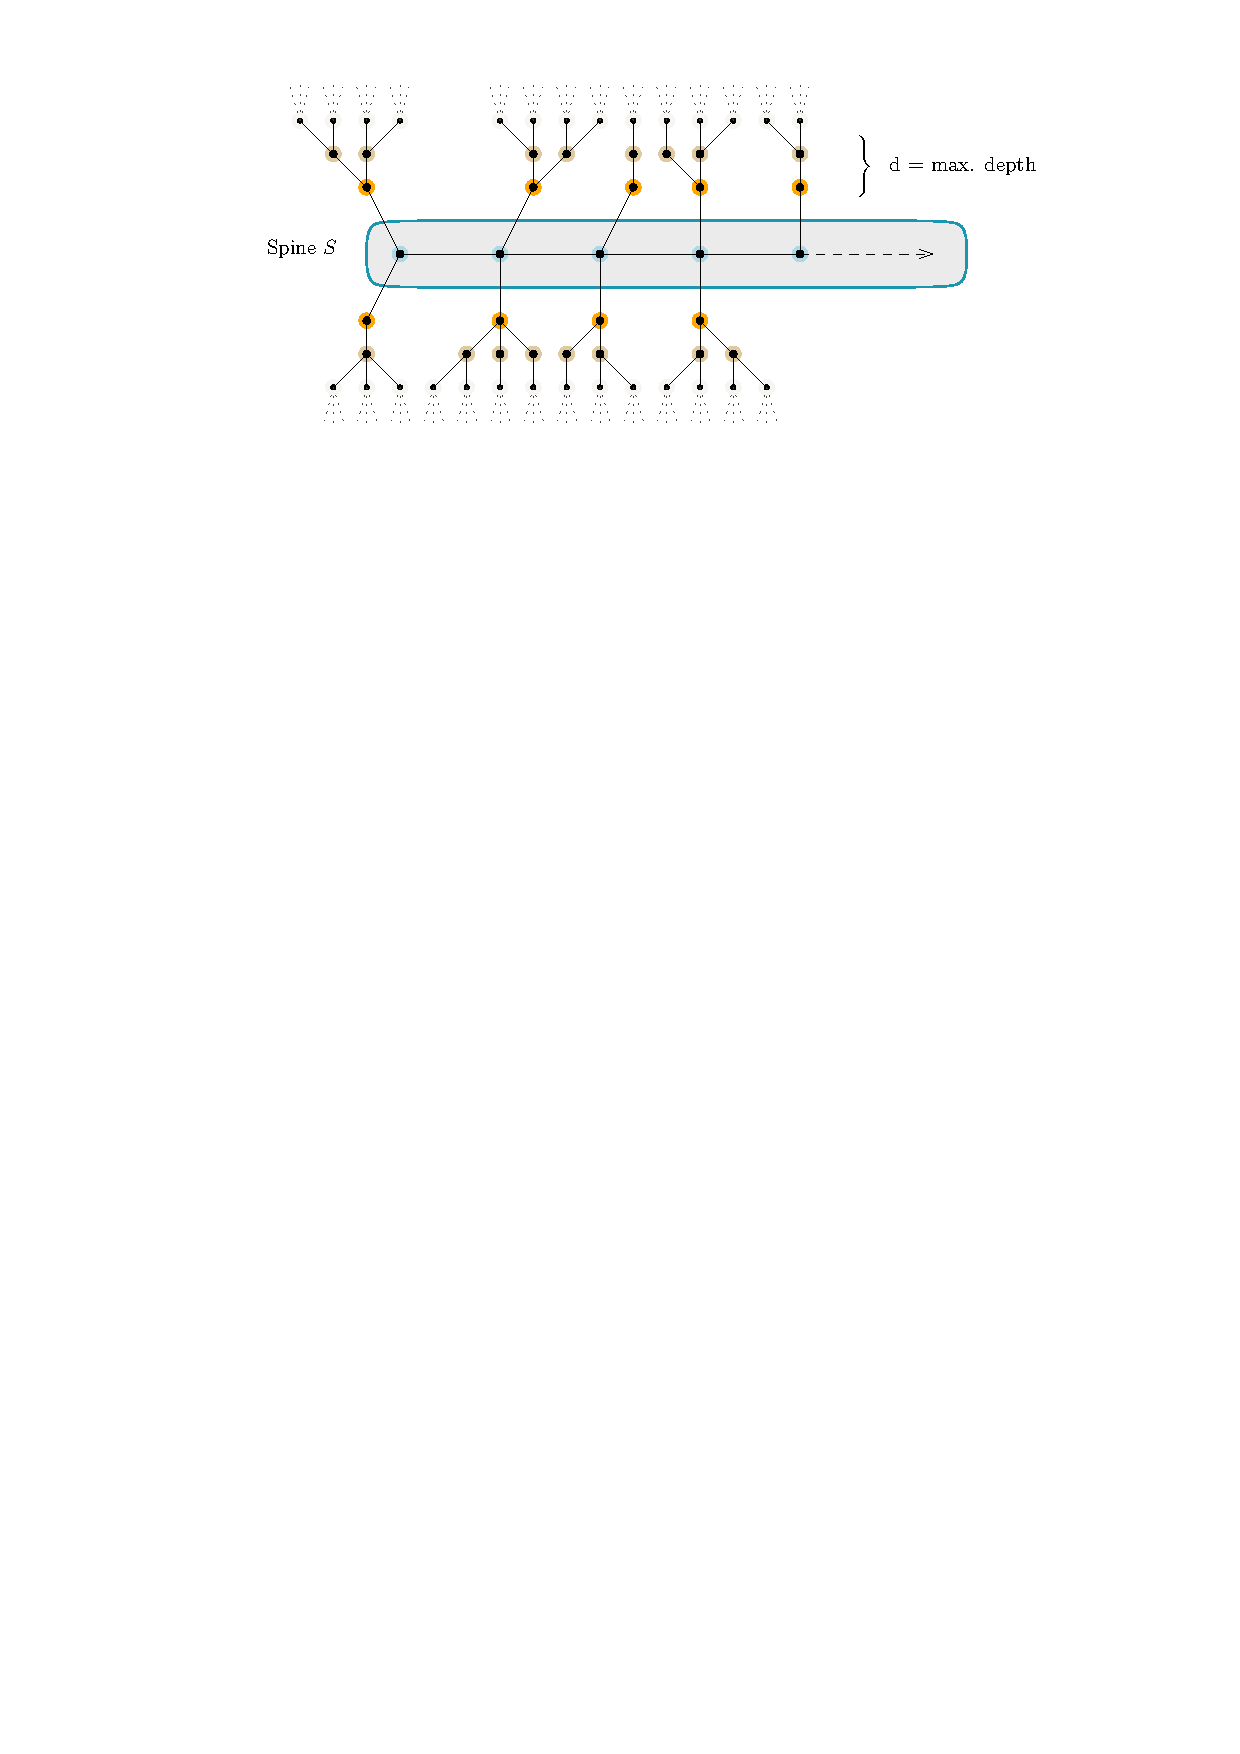
\includegraphics{graphics/ch2_spinedgraph.pdf}
    \caption[Spined graph]{A spined graph consists of a string of vertices identified as the \emph{spine}, here marked in blue. Connected to the spine vertices, we find the subtrees rooted in the orange vertices. All brown vertices have a distance of two to the spine.}
    \label{fig:ch2-spinedgraph}
\end{figure}

A \emph{spined graph} is a tree $G = (\Spines \dotcup \mathcal T, E)$, where $\Spines = \{ s_1, \ldots, s_k \}$ is the set of \emph{spine vertices} and $\mathcal T$ are the \emph{subtree} vertices. The spine is a connected string: $(s_i, s_{i+1}) \in E$. The \emph{depth} $d$ of $G$ is defined as the maximum path distance from any $t \in \mathcal T$ to any spine in $\Spines$. With unbounded depth and unbounded spine length, spined graphs are merely trees with a path designated as the spine. However, by bounding $d$ by a constant, we treat ourselves to a new class of graph, simpler than the general tree. Refer to Figure~\ref{fig:ch2-spinedgraph} for illustration.

A \emph{caterpillar} is a spined graph $(\Spines \dotcup \Leaves, E)$ with depth $d=1$, where $\Leaves$ is the set of \emph{leaves}: vertices at distance $1$ from the spine. Every leaf $l \in \Leaves$ is connected to its parent spine vertex $p(l) \in \Spines$: $(l, p(l)) \in E$.

We are now prepared to introduce the graph class which is the core subject of our examination.

\begin{definition}[Lobster]
A lobster is a spined graph $(\Spines \dotcup \Branches \dotcup \Leaves, E)$ with depth $d=2$, where $\Branches$ is the set of \emph{branches} and $\Leaves$ is the set of \emph{leaves}. Branches have distance $1$ from the spine, leaves have distance $2$.

Every branch $b \in \Branches$ is connected to its parent spine vertex $p(b) \in \Spines$: $(b, p(b)) \in E$. Every leaf $l \in \Leaves$ is connected to its parent branch $p(l) \in \Branches$: $(l, p(l)) \in E$.
\end{definition}

\begin{figure}[b]
    \centering
    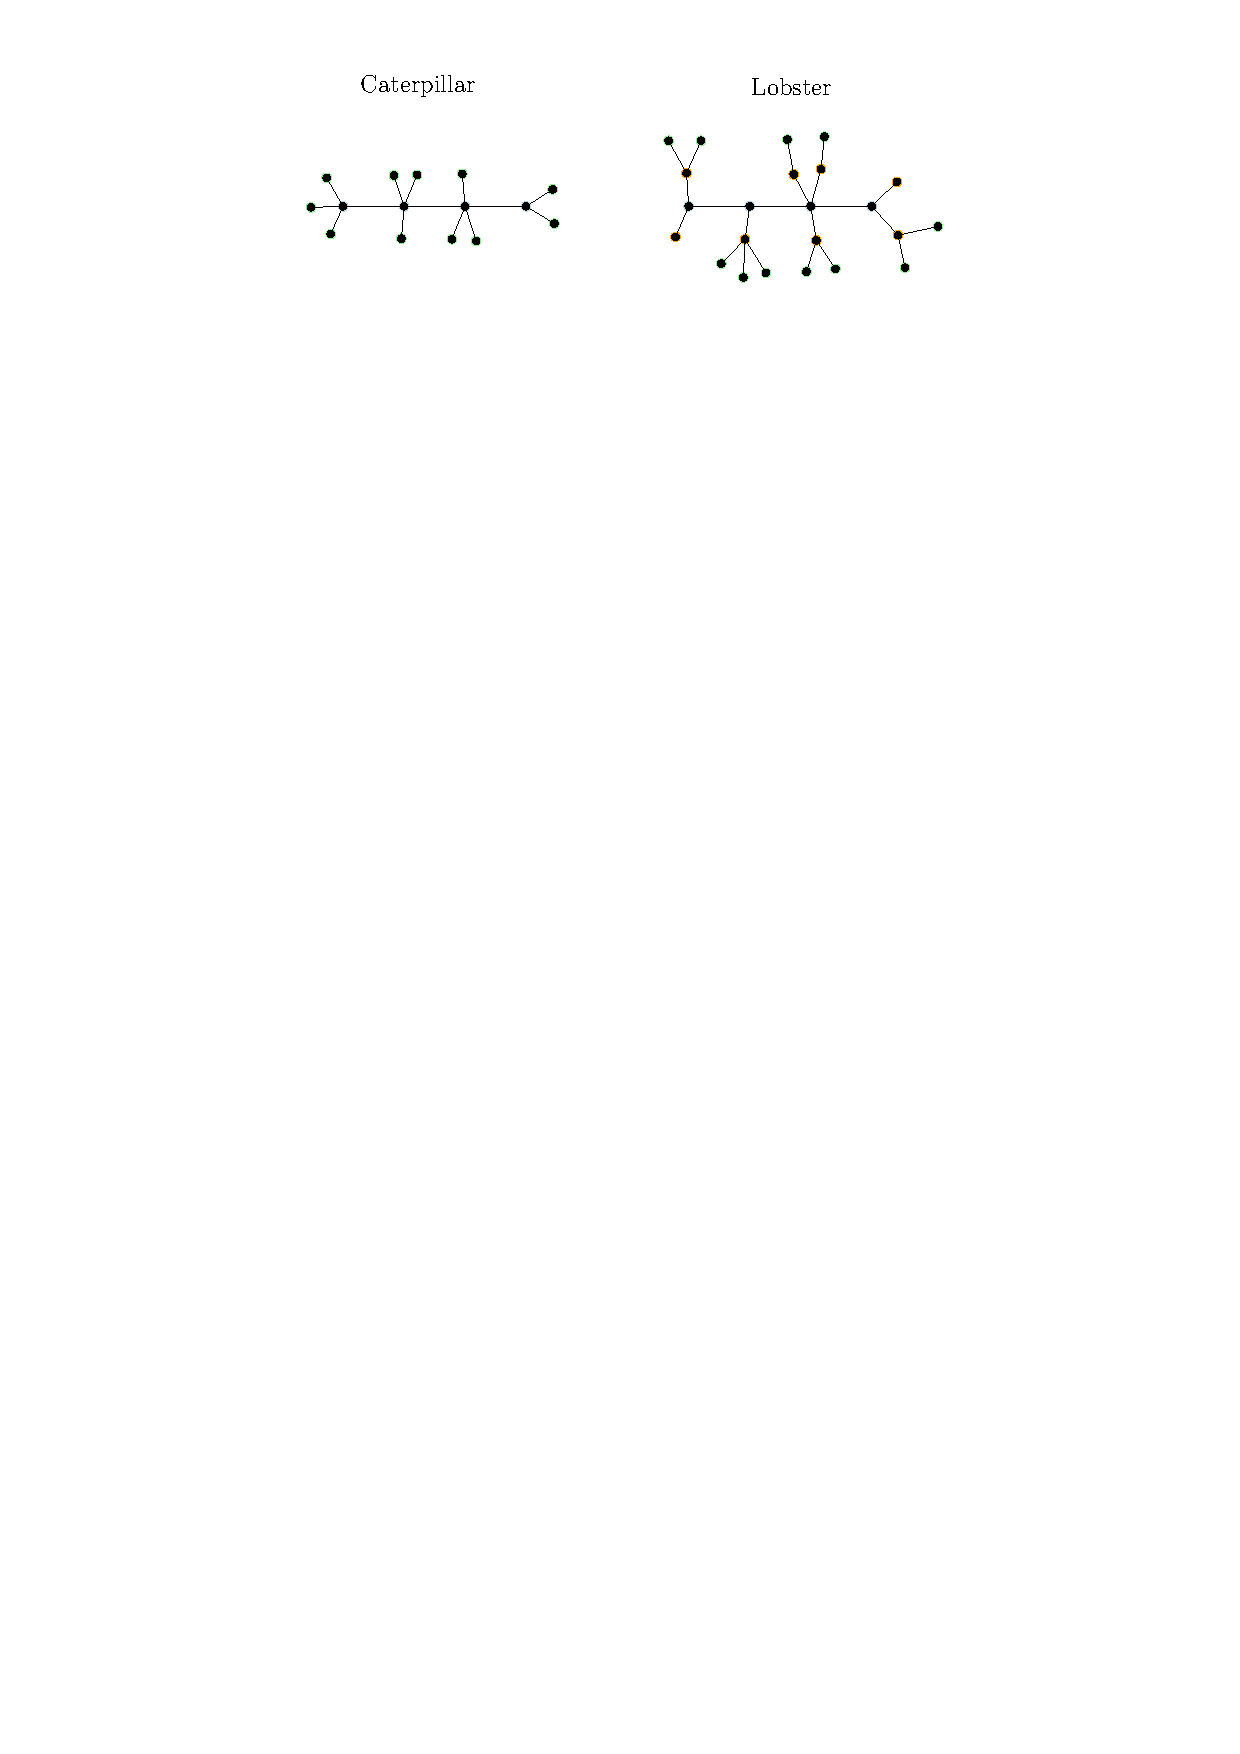
\includegraphics{graphics/ch2_caterpillar_lobster.pdf}
    \caption[Caterpillar and lobster]{The caterpillar (left) and lobster (right) are the only kinds of spined graphs which we explore in this thesis.}
    \label{fig:ch2_caterpillar_lobster}
\end{figure}

Figure~\ref{fig:ch2_caterpillar_lobster} displays a caterpillar and a lobster.

\section{Representations}

A \emph{combinatorial embedding} (or just \emph{embedding}) of a graph in the plane encodes the topological properties of the graph. For each vertex, the embedding defines the clockwise-ordered permutation of its neighbors. The embedding is independent of any specific planar coordinates for vertices and edges, but every drawing of a planar graph induces an embedding.

In this thesis, we define the \emph{embedding function} $d$ over $G$---not to be confused with the embedding, see above---as a bijection $d\colon V \to \reals^2$, which maps vertices to coordinates in the plane. In the common node-link diagram representation, we would draw straight lines to represent the edges. The notation $d$ is short for ``disk'' since we use it to define centers of disks.

The \emph{Euclidean norm} $||v||, v = (v_x, v_y)$, is the length of the vector $v \in \reals^2$, calculated as $||v|| = \sqrt{v_x^2 + v_y^2}$. We denote the distance between the points $v_1$ and $v_2$ by $||v_1 - v_2||$.

The most common notions of graph drawings represent vertices as points. Numerous alternative representations exist. We are particularly interested in drawings with vertices represented as disks.

\begin{definition}[Disk Contact Representation]
\label{def:ch2_DCR}
Let $G = (V, E)$ be a graph and $d$ be an embedding function over $G$. Further let $w\colon V \to \reals$ be a \emph{weight function} for the vertices of $G$ such that

\begin{align*}
\lVert d(v_1) - d(v_2) \rVert &= \frac12(w(v_1) + w(v_2)) &\text{ if } (v_1, v_2) \in E \text{ and} \\ \lVert d(v_1) - d(v_2) \rVert &> \frac12(w(v_1) + w(v_2)) &\text{ otherwise.}
\end{align*}

Then $D = (d, w)$ is a \emph{disk contact representation} of $G$.
\end{definition}

Note that this definition uses strict inequality for non-edges. Disks of disconnected vertices do not touch. In the next definition, the inequality is relaxed. Disks may touch even if there is no edge between them.

\begin{definition}[Weak Disk Contact Representation]
\label{def:ch2_WDCR}
Let $G = (V, E)$ be a graph, $d$ be an embedding function over $G$ and $w$ be a weight function for $V$ such that

\begin{align*}
\lVert d(v_1) - d(v_2) \rVert &= \frac12(w(v_1) + w(v_2)) &\text{ if } (v_1, v_2) \in E \text{ and} \\ \lVert d(v_1) - d(v_2) \rVert &\ge \frac12(w(v_1) + w(v_2)) &\text{ otherwise.}
\end{align*}

Then $D = (d, w)$ is a \emph{weak disk contact representation} of $G$.
\end{definition}

When we want to explicitly refer to the contact notion from Definition~\ref{def:ch2_DCR}, in contrast to the weak contact from Definition~\ref{def:ch2_WDCR}, we call it \emph{strict} or \emph{proper} contact. In the rest of this thesis, we mainly concern ourselves with weak contact. Thus, the weak contact notion is assumed as the default in every context from now on unless explicitly specified otherwise. Regardless, the further definitions involving disk contact can be used both with weak and strict notions of contact.

$G$ is a \emph{disk contact graph} if it admits a disk contact representation. A disk contact graph can be drawn by drawing for each vertex $v$ a disk centered at $d(v)$ with diameter $w(v)$. The disk of $v$ precisely touches the disks of neighbouring vertices. In a drawing using disks, there are no curves to represent the edges beyond the disks being in contact or not. Note that every strict disk contact graph is also a weak disk contact graph.

Let $G = (\Spines \dotcup \mathcal T, E), \Spines = \{ s_1, \ldots, s_n \}$ be a spined graph and $D = (d, w)$ be a disk contact representation. $D$ is \emph{x-monotone} if $\forall i > 1: d_x(s_{i+1}) > d_x(s_i),$ where $d_x(v)$ is the x-component of the embedded coordinates $d(v)$. Informally, the spine ``goes from left to right''.

If it holds for the weight function $w$ of a disk contact representation of $G = (V, E)$ that $\forall v\in V: w(v) = 1$, then we call it a \emph{unit disk contact representation}, shortening ``unit disk contact'' to UDC for readability. $G$ is a UDC graph or UDCG.

\begin{figure}
    \centering
    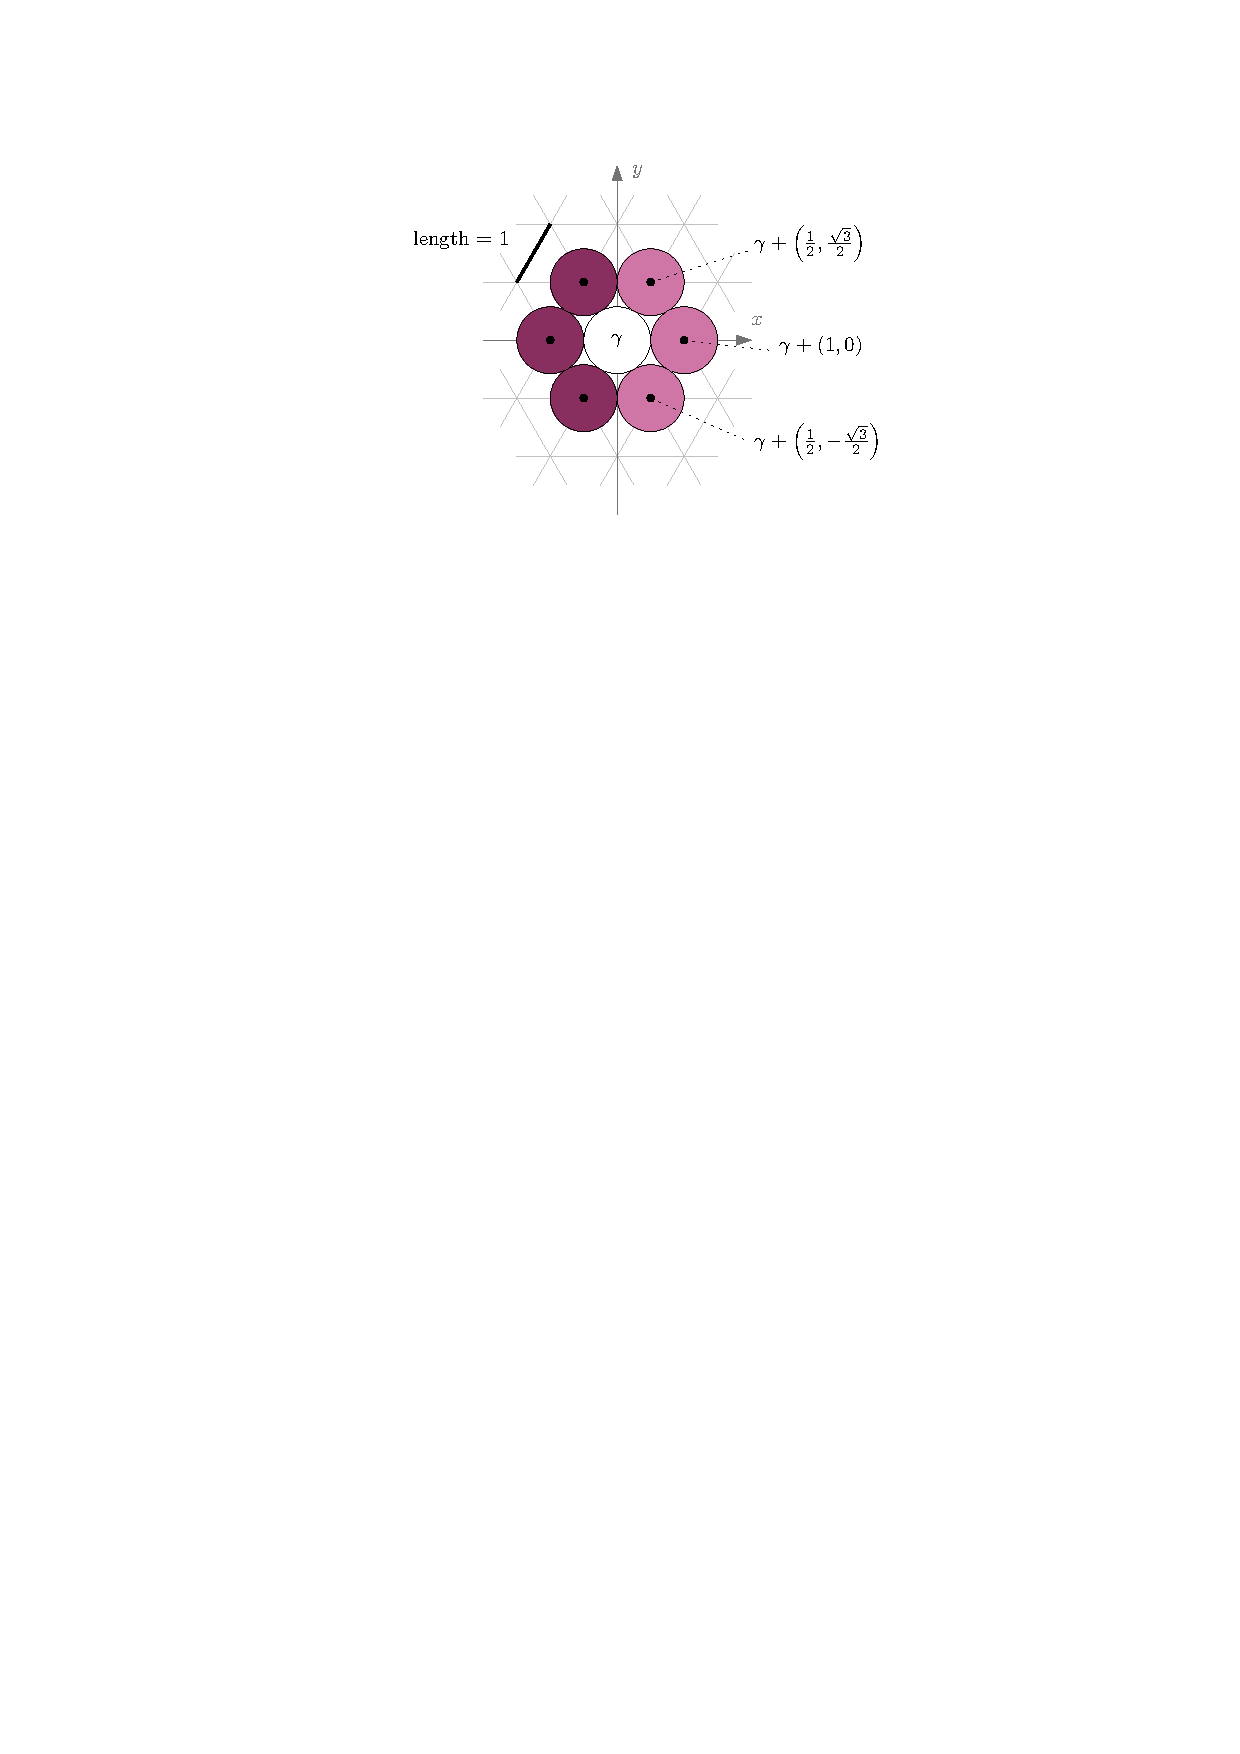
\includegraphics{graphics/ch2_neighborhood.pdf}
    \caption[Tri-grid neighborhood]{The neighborhood $\Gamma(\coord)$ on the triangular grid contains the center coordinates of all purple disks. The x-monotone neighborhood $\Gamma^{x+}(\coord)$ contains only the centers of the light purple disks. All grid distances are unit.}
    \label{fig:ch2-neighborhood}
\end{figure}

Let $D = (d, w)$ be a weak disk contact representation in which $d$ maps all vertices to points from the set $\{ (x + \frac y2, \frac{\sqrt3}2 y) \mid x, y \in \mathbb Z \}$. This set describes the intersection points of a \emph{triangular grid} in the plane, and we call $D$ a \emph{tri-grid representation}. Every such grid point $\coord$ has a \emph{neighborhood}. Using the notation $(\cdot)_{\reals^2}\colon \mathbb C \to \reals^2$ for the bijection $(x + yi)_{\reals^2} = (x, y)$, we define the neighborhood of $\coord$ as the set of points offset from $\coord$ by the sixth unit roots in $\mathbb C$.

\begin{align*}
\Gamma(\coord) = \{ \gamma + (x + yi)_{\reals^2} \mid (x + yi)^6 = 1 \}
%\Bigg\{ &\coord + (-1, 0); \coord + \left(-\frac12, \frac{\sqrt3}2\right); \coord + \left(\frac12, \frac{\sqrt3}2\right);\\
%&\coord + (1, 0); \coord + \left(\frac12, -\frac{\sqrt3}2\right); \coord + \left(-\frac12, -\frac{\sqrt3}2\right) \Bigg\}.
\end{align*}

The more restricted \emph{x-monotone neighborhood}
\begin{align*}\Gamma^{x+}(\coord) = \{ \gamma + (x + yi)_{\reals^2} \mid (x + yi)^6 = 1 \wedge x > 0 \}
%\left\{ \coord + \left(\frac12, \frac{\sqrt3}2\right); \coord + (1, 0); \coord + \left(\frac12, -\frac{\sqrt3}2\right) \right\}
\end{align*}
includes only those neighbors with a larger x-coordinate than $\coord$. Figure~\ref{fig:ch2-neighborhood} illustrates both.

The triangular grid lends itself to UDC representations because the distance between two neighbor coordinates on the triangular grid is exactly $1$. Consequently, unit disks embedded at neighboring tri-grid points are in contact. So, if $G = (V, E)$ is a disk contact graph, $D = (d, w)$ is a UDC representation, $v \in V, \coord = d(v)$ and $(v, u) \in E$, then $d(u) \in \Gamma(\coord)$.

\section{Problems}
\label{section:ch2-problems}

A \emph{recognition problem} is a computational problem in which the goal is to find an algorithm that decides, for a given input from a larger domain, whether that input belongs to a certain smaller class or set in the domain. We say that the algorithm \emph{recognizes} the set.

The broadest problem that we are interested in discussing here is, in the following two variants:

\begin{problem}[Strict UDC Recognition]
Given a graph $G$, does $G$ admit a strict UDC representation?
\label{prob:strict-udc}
\end{problem}

\begin{problem}[Weak UDC Recognition]
Given a graph $G$, does $G$ admit a weak UDC representation?
\label{prob:weak-udc}
\end{problem}

These problems are successors to the original disk contact problem, answered by the above mentioned circle packing theorem. Now restricted to unit size disks, solutions to these problems already exist for the restricted graph class of caterpillars~\cite{Klemz2015,Cleve2020}, which are discussed in Chapter~\ref{chp:related-work}.

As promised in the introduction, we now tie into current research by focusing our attention on the subclass of lobsters. Under the current state of knowledge, we have no algorithm to answer Problems~\ref{prob:strict-udc} or~\ref{prob:weak-udc} in polynomial time, even when the input is restricted to lobsters. We can, however, make some concessions in the form of assumptions to pull the problem into our analytic reach~\cite{Bhore2021}.

\begin{problem}[Tri-Grid X-Monotone UDC Recognition for Lobsters]
Given a lobster $G$, does $G$ admit a weak x-monotone UDC representation on the triangular grid?
\label{prob:weak-udc-lobster}
\end{problem}

Unit disks on the triangular grid are packed decently dense. Disk packing is an entirely own field of research. It is not obvious that every lobster which admits a weak UDC also admits a weak UDC on the triangular grid. This remains an open question. Regardless, the convenience of the triangular grid is ``unlocked'' by and motivates our use of the weak contact notion.

%Unit disks on the triangular grid are packed decently dense. Tighter packing configurations exist, but because this grid is nice and regular and our relevant spine graphs---lobsters---only extend up to two neighbors from the spine, we can assume that the slightly sub-optimal density of our chosen packing configuration does not impact our results compared to the arbitrary configuration. In other words, it is an open question whether a given lobster $G$ admits a tri-grid weak UDC representation if it admits any weak UDC representation. Regardless, the convenience of the triangular grid is ``unlocked'' by and motivates our use of the weak contact notion.

Likewise, we allow ourselves the restriction to x-monotone solutions based on the unproven assumption that a given lobster $G$ admits an x-monotone UDC representation if it admits any UDC representation\footnote{This assumption is the same as in the the proof of linear time for monotone weak UDCs by Bhore et al.~\cite{Bhore2021}.}. As there is no combinatorial embedding prescribed for $G$, no branch necessarily has to be above or below the spine. Yet, to refute our x-monotonicity assumption, a counter-example lobster would have to have some configuration of branches and leaves such that all its possible UDC representations enforce either an acute ($60^\circ$) ``bend'' in the spine, or two consecutive obtuse ($120^\circ$) bends in the same direction. By superficial experimentation, no such configuration has been found so far. The lobster drawn in Figure~\ref{fig:ch2_tri-grid_x-monotone} does admit a tri-grid x-monotone representation.

If our assumptions should hold, then solving Problem~\ref{prob:weak-udc-lobster} is equivalent to solving Problem~\ref{prob:weak-udc}. Hence we focus our aims on Problem~\ref{prob:weak-udc-lobster}.

With the subject problem properly outlined, we explore the current state of research on the following questions:

\begin{enumerate}
    \item[Question 1:] Can we decide the weak UDC recognition problem for lobsters of size $n$ in time $O(n)$?
    \item[Question 2:] Can we decide the tri-grid x-monotone UDC recognition problem for lobsters of size $n$ in time $O(n)$?
\end{enumerate}

\begin{figure}
    \centering
    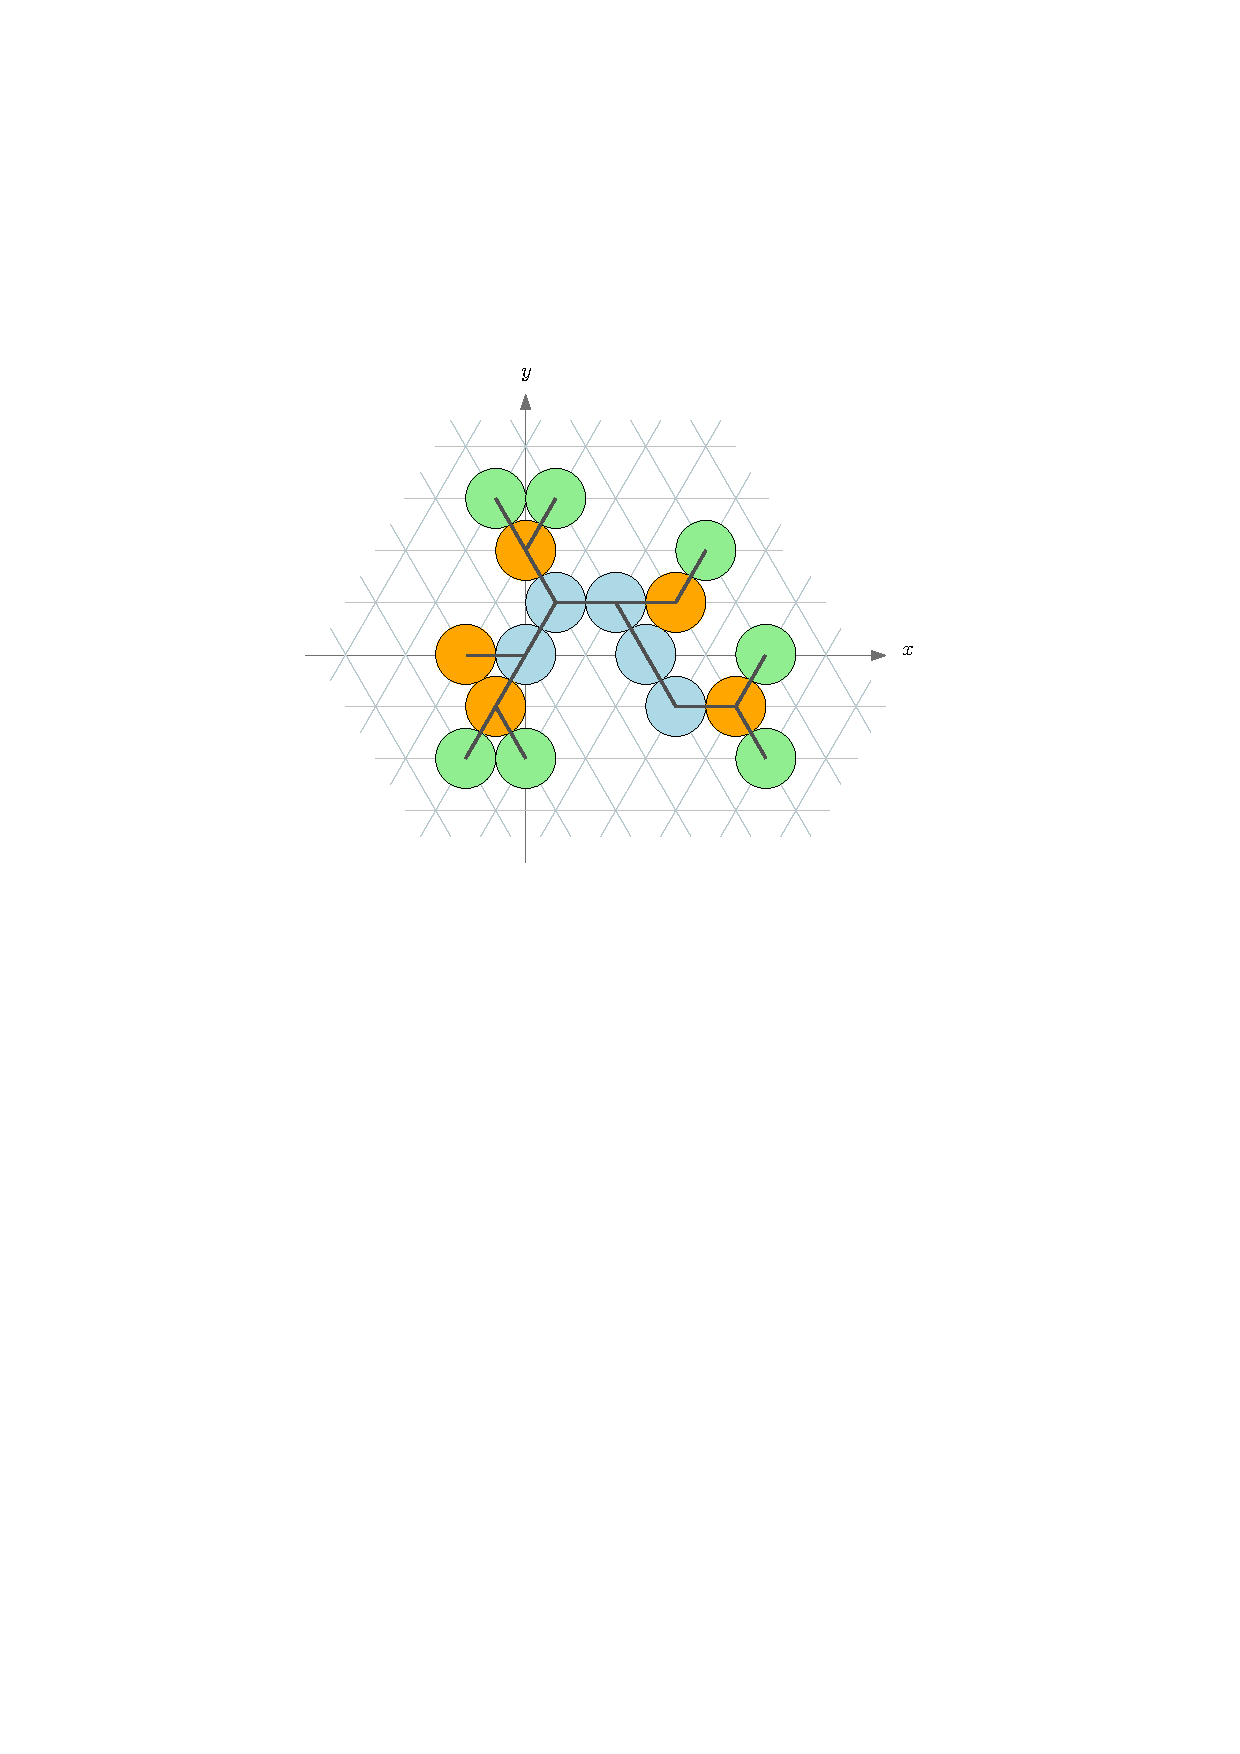
\includegraphics{graphics/ch2_tri-grid_x-monotone.pdf}
    \caption[Tri-grid x-monotone UDC representation of a lobster]{A tri-grid x-monotone UDC representation of a lobster. Spine, branch and leaf vertices are mapped to the blue, orange and green disks respectively. The spine, although it bends twice, is embedded on strictly increasing x-coordinates.}
    \label{fig:ch2_tri-grid_x-monotone}
\end{figure}
